\documentclass[]{article}
\usepackage[utf8]{inputenc}
\usepackage{hyperref}
\usepackage[spanish]{babel}
\usepackage{listings}
\usepackage{xcolor} %para el texto con coloresç
\usepackage{tocloft}
\usepackage{graphicx}

\usepackage[colorinlistoftodos,prependcaption,textsize=tiny]{todonotes}

\renewcommand{\cftsecleader}{\cftdotfill{\cftdotsep}} % Para que todo el índice tenga puntos
\newcommand{\code}[1]{{\lstinline[basicstyle=\ttfamily,mathescape]!#1!}}
\newcommand{\toolname}{\emph{Tutoriales Interactivos}}

\lstset{ %
	%backgroundcolor=\color{white},  % choose the background color; you must add \usepackage{color} or \usepackage{xcolor}
	basicstyle=\sffamily,      % the size of the fonts that are used for the code
	breakatwhitespace=false,         % sets if automatic breaks should only happen at whitespace
	breaklines=true,                 % sets automatic line breaking
	captionpos=none,                 % sets the caption-position to bottom
	commentstyle=\itshape\color{gray},           % comment style
	%deletekeywords={...},           % if you want to delete keywords from the given language
	escapeinside={(*}{*)},           % if you want to add LaTeX within your code
	extendedchars=true,              % lets you use non-ASCII characters; for 8-bits encodings only, does not work with UTF-8
	frame=tb,	                   % adds a frame around the code
	keepspaces=true,                 % keeps spaces in text, useful for keeping indentation of code (possibly needs columns=flexible)
	columns=fullflexible,
	%keywordstyle=\color{blue},      % keyword style
	 keywordstyle=\sffamily\color{teal},
	numbers=left,                    % where to put the line-numbers; possible values are (none, left, right)
	numbersep=5pt,                   % how far the line-numbers are from the code
	numberstyle=\tiny, % the style that is used for the line-numbers
	%rulecolor=\color{black},         % if not set, the frame-color may be changed on line-breaks within not-black text (e.g. comments (green here))
	showspaces=false,                % show spaces everywhere adding particular underscores; it overrides 'showstringspaces'
	showstringspaces=false,          % underline spaces within strings only
	showtabs=false,                  % show tabs within strings adding particular underscores
	stepnumber=1,                    % the step between two line-numbers. If it's 1, each line will be numbered
	stringstyle=\color{blue},     % string literal style
	tabsize=2,	                   % sets default tabsize to 2 spaces
	title=\lstname,                   % show the filename of files included with \lstinputlisting; also try caption instead of title	
	mathescape=true
}

\lstdefinelanguage{yaml}{
	%backgroundcolor=\color{white},  % choose the background color; you must add \usepackage{color} or \usepackage{xcolor}
	basicstyle=\ttfamily,      % the size of the fonts that are used for the code
	breakatwhitespace=false,         % sets if automatic breaks should only happen at whitespace
	breaklines=true,                 % sets automatic line breaking
	captionpos=none,                 % sets the caption-position to bottom
	commentstyle=\sffamily\color{gray},           % comment style
	%deletekeywords={...},           % if you want to delete keywords from the given language
	escapeinside={(*}{*)},           % if you want to add LaTeX within your code
	extendedchars=true,              % lets you use non-ASCII characters; for 8-bits encodings only, does not work with UTF-8
	frame=tb,	                   % adds a frame around the code
	keepspaces=true,                 % keeps spaces in text, useful for keeping indentation of code (possibly needs columns=flexible)
	columns=fullflexible,
	%keywordstyle=\color{blue},      % keyword style
	%language=C++,                 % the language of the code
	numbers=left,                    % where to put the line-numbers; possible values are (none, left, right)
	numbersep=5pt,                   % how far the line-numbers are from the code
	numberstyle=\tiny, % the style that is used for the line-numbers
	%rulecolor=\color{black},         % if not set, the frame-color may be changed on line-breaks within not-black text (e.g. comments (green here))
	showspaces=false,                % show spaces everywhere adding particular underscores; it overrides 'showstringspaces'
	showstringspaces=false,          % underline spaces within strings only
	showtabs=false,                  % show tabs within strings adding particular underscores
	stepnumber=1,                    % the step between two line-numbers. If it's 1, each line will be numbered
	%stringstyle=\color{mymauve},     % string literal style
	tabsize=2,	                   % sets default tabsize to 2 spaces
	title=\lstname,                   % show the filename of files included with \lstinputlisting; also try caption instead of title	
	mathescape=true,
	comment=[l]{\#}
}

% Title Page
\title{\toolname{} -- Creación de lecciones}
\author{Enrique Martín Martín (\url{emartinm@ucm.es}) \\ \emph{Revisor:} Nombre Apellidos (\url{correo@ucm.es})\\~\\[-.4cm]
	\normalsize{Dpto. Sistemas Informáticos y Computación, Fac. Informática}\\[-0.1cm]
    \normalsize{Universidad Complutense de Madrid}}


\begin{document}
\maketitle

\begin{abstract}
La herramienta \toolname{} organiza su contenido en distintas carpetas dentro del \emph{directorio de temas}. Estas carpetas corresponden a cada uno de los lenguajes de programación soportados, y contienen un fichero YAML por cada tema. A su vez, los temas están definidos como una secuencia de lecciones, que contiene distintos elementos. En este documento se explicará la organización de carpetas y el formato concreto de los ficheros de temas.
\end{abstract}

\tableofcontents

\clearpage


\section{Organización de carpetas}
Todo el contenido de la aplicación se almacena en la \emph{carpeta de temas}, cuya localización debe establecer el usuario desde la ventana de configuración. Esta carpeta contendrá un directorio por cada lenguaje para el que se quiera proporcionar temas, aunque pueden existir varios directorios para versiones alternativas del mismo lenguaje de programación (por ejemplo \emph{Python 2.x} y \emph{Python 3.x}, o \emph{OpenJDK 6} y \emph{Oracle Java 8}). Para determinar cuál es el lenguaje de programación asociado a un directorio la herramienta \toolname{} inspecciona su nombre, comprobando si contiene alguna subcadena. Actualmente se soportan 4 lenguajes de programación, y la comprobación de nombre se realiza en el siguiente orden:

\begin{enumerate}
  \item \textbf{Python}: si el nombre del directorio contiene la subcadena \textbf{<<python>>}\footnote{No importa si las subcadenas aparecen en mayúsculas o minúsculas en el nombre del directorio.}. Para cada uno de estos directorios, la ventana de configuración mostrará una entrada para establecer la ruta del intérprete.\todo{igual debería incluirse el interprete esperado como en los siguientes puntos}
  \item \textbf{Java}: si contienen la subcadena \textbf{<<java>>} en su nombre. Para cada uno de estos directorios, la ventana de configuración mostrará dos entradas: una para establecer la ruta del compilador \emph{javac} y otra para establecer la ruta del entorno de ejecución \emph{java}.\todo{unificar formato de los comandos con los siguientes puntos}
  \item \textbf{C++}: si contienen la subcadena \textbf{<<c++>>}. Para cada uno de estos directorios, la ventana de configuración mostrará una entrada para establecer la ruta del compilador \emph{GNU C++} (\code{g++}) o la del fichero de entorno de \emph{Visual Studio} (\code{vcvars*.bat}). 
  \item \textbf{C\#}: si el nombre contiene la subcadena \textbf{<<c sharp>>}. Para estos directorios aparecerá una entrada en la ventana de configuración para establecer la ruta del compilador \emph{Mono} (\code{mcs}) o el fichero de entorno de \emph{Visual Studio} (\code{vcvars*.bat}).
\end{enumerate}

\section{Formato de los temas}
\begin{figure}[tbp]
\begin{lstlisting}[language=yaml,basicstyle=\ttfamily\footnotesize]
Subject: 1
Title: Titulo del tema
Intro: Breve explicaci(*ó*)n del tema
Lessons:
    - Title: Explicaciones #Primera leccion
      Elements: #Lista de elementos de la leccion
          - Elem: Text #Elemento de tipo explicacion (*\label{fig:tema:explicacion}*)
            Content: | #Texto de varias lineas
              Las explicaciones sirven para mostrar informaci(*ó*)n al alumno. (*\label{fig:tema:exp1}*)

              Estas esplicaciones se pueden dividir en varios p(*á*)rrafos, y con 
              Markdown se pueden incluir **negritas**, *it(*a*)licas* y `c(*ó*)digo`. (*\label{fig:tema:exp2}*)
          - Elem: Text
            Content: |
                **Imagen desde internet** (*\label{fig:tema:exp3}*)
                ![texto alternativo](http://URL/imagen.png)

                **Imagen desde el directorio de temas con ruta relativa**
                ![triangulo](file://img/triangulo.jpg)
  
                **Se pueden incluir enlaces en las explicaciones:**
                [Texto del enlace](https://www.ucm.es) (*\label{fig:tema:exp4}*)
    - Title: Preguntas de tipo test #Segunda leccion
      Elements:
          - Elem: Options #Pregunta de varias opciones (*\label{fig:tema:opt1}*)
            Content: Pregunta de 3 opciones y una correcta #Texto de la pregunta
            Hint: Esto es la pista general de la pregunta
            Solution: [1] #Opciones correctas, empezando en 1
            Multiple: no #Hay varias opcinones correctas?
            Options: # Lista de opciones para mostrar
                - OPCI(*Ó*)N CORRECTA
                - Opci(*ó*)n incorrecta
                - Opci(*ó*)n incorrecta (*\label{fig:tema:opt2}*)
    - Title: Preguntas de tipo c(*ó*)digo #Tercera leccion
      Elements:
          - Elem: Code #Pregunta de codigo (*\label{fig:tema:code1}*)
            Content: | #Texto de la pregunta, varias lineas
                Estas preguntas solicitan al usuario framentos de c(*ó*)digo que
                son insertados en una plantilla correctora, que es evaluada.
            Gaps: 2 #Numero de huecos a rellenar
            Prompt: ["Codigo hueco 1","Codigo hueco 2"] #Informacion de cada hueco
            Hint: Esto es la pista general. 
            File: correctores/plantilla.py #Plantilla correctora con 'huecos' (*\label{fig:tema:code2}*)
\end{lstlisting}
\caption{Ejemplo de fichero de tema con tres lecciones y varios elementos en cada lección.\label{fig:tema}}
\end{figure}

Cada directorio que aparece en la carpeta de temas puede contener varios temas. Estos temas se definirán en ficheros con formato \code{YAML}\footnote{\url{http://www.yaml.org/spec/1.2/spec.html}} con extensión \textbf{obligatoria} \code{.yml}. El formato \code{YAML} es similar a \code{JSON} \todo{Se le da un link casi al final, pero igual convendría ponerlo aquí por ser la primera referencia.}y sirve para representar información como texto plano en diccionarios clave-valor, listas y tipos de datos básicos como booleanos, números, cadenas, etc.

Un ejemplo de fichero de tema se puede observar en la Figura~\ref{fig:tema}\todo{creo que sería útil meter YAML por algun lado del caption}, donde se han añadido comentarios de línea (que comienzan con \code{\#}) para aclarar algunos apartados. El formato concreto es un diccionario YAML con las siguientes claves y valores:
\begin{itemize}
\item \code{Subject}: {\sf (OBLIGATORIO)} \textbf{número} de tema. Sirve para ordenar los distintos temas de un lenguaje a la hora de mostrarlos.
\item \code{Title}: {\sf (OBLIGATORIO)} \textbf{cadena de texto} con el título del tema. 
\item \code{Intro}: {\sf (OBLIGATORIO)} \textbf{cadena de texto} que explica brevemente el objetivo del tema. Este texto puede incluir código \emph{Markdown} o incluso código HMTL, como veremos en la Sección~\ref{sec:explicaciones}.
\item \code{Lessons}: {\sf (OBLIGATORIO)} lista de \textbf{lecciones} dentro del tema.
\end{itemize}

Cada una de las lecciones del tema se representa a su vez como diccionarios con dos claves:
\begin{itemize}
\item \code{Title}: {\sf (OBLIGATORIO)} \textbf{cadena de texto} con el título de la lección.
\item \code{Elements}: {\sf (OBLIGATORIO)}  lista de \textbf{elementos} que conforman la lección. Existen tres tipos de elementos: \textbf{explicaciones}, \textbf{preguntas de varias opciones} y \textbf{preguntas de código}. Los distintos elementos se tratarán con detalle en las siguientes secciones.
\end{itemize}

\begin{figure}[tb]
	\centerline{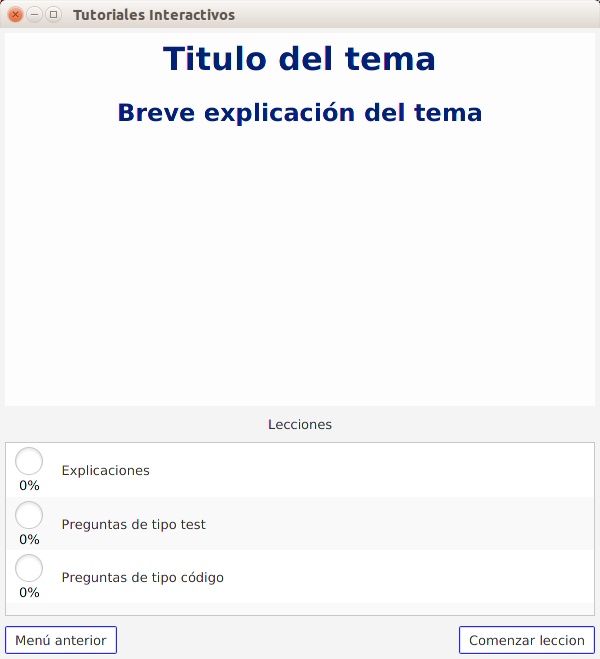
\includegraphics[scale=0.4]{lecciones}}
	\caption{Pantalla de selección de lecciones\label{fig:lecciones}}
\end{figure}

El título de tema, su introducción y los títulos de temas son los que \toolname{} utiliza para mostrar las pantallas de selección de tema y lecciones. En la Figura~\ref{fig:lecciones} se puede ver cómo se mostrarían la pantalla de selección para elegir entre las tres lecciones del tema definido en la Figura~\ref{fig:tema}.


\section{Explicaciones}\label{sec:explicaciones}
\todo{Creo que se podría crear una seccion con "Formato de los elementos de lección", y poner las siguientes 3 secciones como subsecciones.}
Los elementos de tipo \emph{explicación} sirven para mostrar al alumno texto y otros contenidos gráficos. Se representan como un diccionario de dos claves:
\begin{itemize}
	 \item \code{Elem: Text} {\sf (OBLIGATORIO)}
	 \item \code{Content}: {\sf (OBLIGATORIO)} \textbf{cadena de texto} con el contenido que se quiere mostrar. Puede ser texto plano, código Markdown\footnote{\url{https://github.com/adam-p/markdown-here/wiki/Markdown-Cheatsheet}} \todo{por vender la moto se puede comentar que ambos formatos facilitan la exportación a otros medios como wikis, foros (stackoverflow), repositorios online (github), etc. Por darle un valor añadido o reforzar la justificación de la elección de estos formatos.}o código HTML. La opción preferida es código Markdown por ser el más sencillo y ser suficientemente flexible. En la Figura~\ref{fig:tema} se pueden ver ejemplos de contenidos Markdown en las líneas~\ref{fig:tema:exp1}--\ref{fig:tema:exp2} y~\ref{fig:tema:exp3}--\ref{fig:tema:exp4}
\end{itemize}

\subsection{Markdown}
\todo{Creo que esto podría ponerse antes como sección como "Formatos de texto aceptados' o algo así, y después ya introducir las cosas especificas de cada tipo de elemento de lección. }
Markdown proporciona muchas características para dar formato a un texto. La herramienta \toolname{} soporta como mínimo las siguientes:
\begin{itemize}
	\item \textbf{Negrita, itálica y código integrado en la línea}:
\begin{lstlisting}[language=yaml,numbers=none]
**negrita**, *italica*, `codigo de una linea`
\end{lstlisting}	
	\item \textbf{Bloques de código de varias lineas}:
\begin{lstlisting}[language=yaml,numbers=none]
```
def f(n):
    return n + 1
```
\end{lstlisting}
	\item \textbf{Cabeceras de sección}:
\begin{lstlisting}[language=yaml,numbers=none]
(*\# Cabecera 1*)
bla bla bla

(*\#\# Cabecera 2*)
bla bla bla

(*\#\#\# Cabecera 3*)
bla bla bla

\end{lstlisting}
	\item Listas numeradas y no numeradas:
\begin{lstlisting}[language=yaml,numbers=none]
* Elemento no numerado 1
    1. elemento numerado anidado 1
    1. elemento numerado anidado 2
    1. elemento numerado anidada 3
* Elemento no numerado 2
    * elemento no numerado anidado 1
    * elemento no numerado anidado 2 
\end{lstlisting}	
	\item \textbf{Imágenes}: pueden ser imágenes remotas o almacenadas en el directorio del tema.
\begin{lstlisting}[language=yaml,numbers=none]
**Imagen remota**
![texto alternativo](https://URL/imagen.png)

**Imagen desde el directorio de temas, con ruta relativa**
![triangulo](file://img/triangulo.jpg)
\end{lstlisting}		
Todas las imágenes cuya ruta comience con \code{file://} serán consideradas imágenes locales cuya ruta es relativa al directorio donde reside el tema actual. Por ejemplo, si el tema actual reside en <<\code{/opt/temas/Python 3.x}>>, la imagen <<\code{file://img/triangulo.jpg}>> se referirá al fichero situado en <<\code{/opt/temas/Python 3.x/img/triangulo.jpg}>>.
	\item \textbf{Enlaces} que se abren en el navegador por defecto:
\begin{lstlisting}[language=yaml,numbers=none]
[Texto del enlace](https://www.ucm.es)
\end{lstlisting}
	\item \textbf{Notación matemática \LaTeX}. Gracias el entorno MathJax\footnote{\url{https://www.mathjax.org/}} es posible incrustar código \LaTeX{} en el texto. El código \LaTeX{} debe encerrarse entre los símbolos \code{@@} para fórmulas en la misma línea y \code{@@@} para fórmulas en párrafos nuevos:
\begin{lstlisting}[language=yaml,numbers=none]
Consideremos el polinomio @@ax^2 + bx + c = 0@@
Cuando @@a \ne 0@@, existen dos soluciones:
@@@x = {-b \pm \sqrt{b^2-4ac} \over 2a}.@@@	
\end{lstlisting}
	\item \textbf{Tablas}:
\begin{lstlisting}[language=yaml,numbers=none]
Cabecera|Cabecera|Cabecera
:-------|:------:|-------:  #Distintos tipos de alineacion horizontal
 1      | 2      | 3
 1      | 2      | 3
\end{lstlisting}	
\end{itemize}

\begin{figure}[tb]
	\centerline{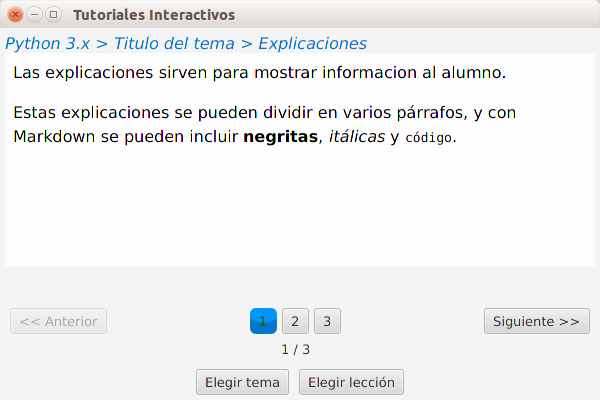
\includegraphics[scale=0.5]{explicacion}}
	\caption{Pantalla mostrando la primera explicación de la lección <<Explicaciones>>\label{fig:explicacion}}
\end{figure}

La Figura~\ref{fig:explicacion} muestra cómo se mostraría la primera explicación definida en la línea~\ref{fig:tema:explicacion} \todo{hasta la línea ayudaría (aunque es obvío)}de la Figura~\ref{fig:tema}, que contiene dos párrafos y texto en negrita, itálica y monoespaciado. Recomendamos consultar el <<Tema de prueba>> que se puede encontrar en \url{https://github.com/emartinm/TutorialesInteractivos/blob/master/temas/Python%203.x/Tema0.yml} para ver en detalle las distintas características Markdown que se han presentado en esta sección.

\subsection{HMTL}
En aquellas situaciones donde Markdown no es suficiente, se puede incluir código HMTL directamente. Esto puede servir para incrustar vídeos y otros elementos interactivos.\footnote{La herramienta \toolname{} utiliza internamente la componente \emph{WebView} de JavaFX, que está basada en WebKit (\url{https://webkit.org/}). Por lo tanto, la capacidad para procesar HTML será algo menor al de los navegadores de escritorio usuales y habrá algunas características que no funcionen correctamente o directamente no estén soportadas.} Por ejemplo el siguiente código incrustaría el vídeo \url{https://www.youtube.com/embed/PDpMgx7avzA} como un \code{iframe}:
\begin{lstlisting}[language=yaml,numbers=none]
<iframe width="640" height="360" src="https://www.youtube.com/embed/PDpMgx7avzA" frameborder="0" allowfullscreen target="_self"></iframe>
\end{lstlisting}		

\section{Preguntas de varias opciones}
Este tipo de elementos sirve para preguntas en las que el alumno debe elegir la opción u opciones correctas entre varias disponibles. En el fichero YAML las preguntas de varias opciones se representan como un diccionario con las siguientes claves y valores:\todo{se hace un poco incomodo tener que subir cada vez arriba a buscar la figura 1 para ver el ejemplo. Una opción podría ser poner un mínimo en la figura 1 y desarrollar más en cada una de las secciones. También se puede poner como una apéndice la completa y poner solo las partes implicadas durante la explicación. También ayudaría a hacer más fácil el matching entre las ventanas de las preguntas y su código. }
\begin{itemize}
	\item \code{Elem: Options} {\sf (OBLIGATORIO)}
	\item \code{Content:} {\sf (OBLIGATORIO)} \textbf{cadena de texto} con el enunciado de la pregunta. Al igual que en las explicaciones, este texto puede contener código Markdown o HTML. 
 	\item \code{Hint:} {\sf (OPCIONAL)} \textbf{cadena de texto} con una pista sobre la solución a la pregunta que el alumno puede visualizar pulsando el botón <<Pistas>>.\todo{Esto me hace preguntarme si las pistas deberían penalizar y si se podría dar aquí una opción con un booleano para indicarlo. Esto implicaría también tener 3 grados de estado de una pregunta: sin responder, respondida con pista y respondida. Supongo que es mucho lío, pero pienso que molaría :D}\todo{Molaría que la pista saliera en la ventana de ejemplo.}
 	\item \code{Options:} {\sf (OBLIGATORIO)} \textbf{lista de cadenas} con las distintas opciones que se mostrarán al alumno.\todo{No se comenta nada de los guiones que veo que tiene cada opción al principio.}
 	\item \code{Multiple:} {\sf (OPCIONAL)} \textbf{booleano} que indica si la pregunta puede tener cualquier número de opciones válidas (\code{yes}) o si únicamente una opción será la correcta (\code{no}). En caso de no incluir esta clave, el valor por defecto es \code{no}.\todo{No queda claro si al tener más de una respuesta correcta se han de seleccionar todas las correctas o con marcar alguna ya es válido. }
 	\item \code{Solution:} {\sf (OBLIGATORIO)} \textbf{lista de números} con las posiciones de las opciones correctas, donde la primera opción tiene posición \code{1}. Este campo puede contener la lista vacía (\code{[]}) si ninguna opción es correcta.\todo{Me da la sensación que el anterior campo se puede inferir con este y es innecesario. Si hay más de un elemento en esta lista pues es multiple :).}\todo{Me deja preguntándome que pasa si la lista es vacía. ¿Como superarías la pregunta? }
\end{itemize}

\begin{figure}[tb]
	\centerline{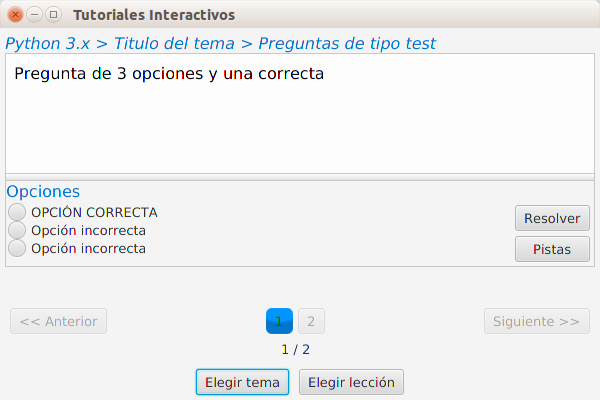
\includegraphics[scale=0.5]{opciones}}
	\caption{Pantalla mostrando una pregunta de tres opciones con solución única.\label{fig:opciones}}
\end{figure}

Las lineas~\ref{fig:tema:opt1}--\ref{fig:tema:opt2} de la Figura~\ref{fig:tema} contienen un ejemplo de pregunta de tres opciones donde únicamente la primera es correcta. A la hora de mostrar esta pregunta, \toolname{} generaría la pantalla de la Figura~\ref{fig:opciones}.

\section{Preguntas de código}
Las preguntas de tipo código permiten solicitar al alumno uno o varios fragmentos de código y evaluar su resultado. Para dicha evaluación los fragmentos de código introducidos por el alumno se insertan en los \emph{huecos} definidos en una \emph{plantilla correctora}\todo{Este concepto no lo pillo a estas alturas}, que está escrita en el mismo lenguaje de programación que está aprendiendo el alumno. Esta plantilla se rellena y se ejecuta para obtener su veredicto, lo que involucra distintas fases dependiendo del lenguaje de programación: invocar directamente al intérprete (Python), compilar la plantilla rellena y luego invocar el binario generado (C++ y C\#), compilar la plantilla rellena y luego interpretar el fichero generado (Java). La estructura de las plantillas correctoras se detallará en la Sección~\ref{sec:plantillas}.

En el fichero YAML las preguntas de código se representan como un diccionario con las siguientes claves y valores:\todo{Si el orden en el que se introducen las claves-valores no es importante (igual debería decirse en algún sitio), entonces se podría dividir en dos grupos: obligatorios y opcionales. Creo que se vería más claro y facilitaría el probar la herramienta de manera rápida.}
\begin{itemize}
	\item \code{Elem: Code} {\sf (OBLIGATORIO)}
	\item \code{Content:} {\sf (OBLIGATORIO)} \textbf{cadena de texto} con el enunciado de la pregunta. Como es usual, este texto puede contener código Markdown o HTML. 
	\item \code{Gaps:} {\sf (OPCIONAL)} \textbf{número entero} ($> 0$) que indica el número de huecos que debe rellenar el alumno. Si no se incluye este campo, el valor por defecto es $0$.	
	\item \code{Prompt:} {\sf (OPCIONAL)} \textbf{lista de cadenas de texto} con tantos elementos como se indique en el campo \code{Gaps}. Indica el texto por defecto que debe aparecer en cada campo de texto cuando está vacío. Sirve para dar indicaciones al alumno sobre lo que debe introducir en cada hueco.\todo{que pasa si hay discrepancias entre los valores gaps y prompt. Si por ejemplo digo 1 gap y pongo una lista con 3 prompts. O pongo 3 gaps y solo defino 1 prompt? igual Gaps es prescidible y con prompt es suficiente. Si defines una lista [<<>>, <<>>, <<>>] es que no quieres prompts pero quieres 3 gaps.}
	\item \code{Hint:}  {\sf (OPCIONAL)} \textbf{cadena de texto} con una pista sobre la solución a la pregunta que el alumno puede visualizar pulsando el botón <<Pistas>>.\todo{molaría verla en la ventana.}
	\item \code{File:} {\sf (OBLIGATORIO)} \textbf{cadena de texto} con la ruta de la plantilla correctora \emph{relativa al directorio en el que está el tema actual}. Por ejemplo, si el tema actual está en el directorio <<\code{/opt/temas/Python 3.x}>> y la ruta de la plantilla correctar es <<\code{correctores/tema1_p3.py}>>, la ruta completa de la plantilla será <<\code{/opt/temas/Python 3.x/correctores/tema1_p3.py}>>.
\end{itemize}

\begin{figure}[tb]
	\centerline{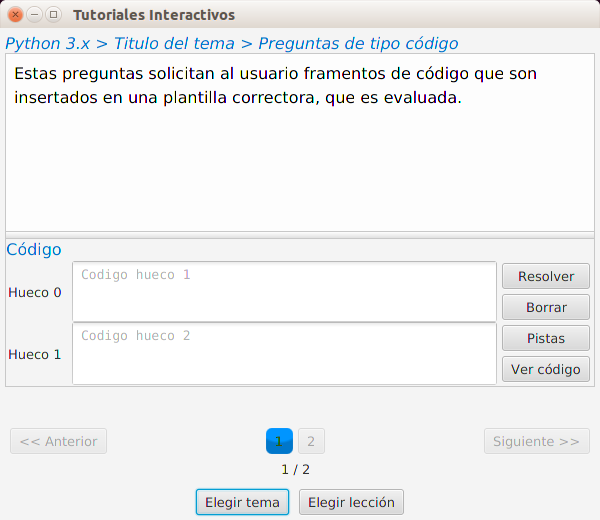
\includegraphics[scale=0.5]{codigo}}
	\caption{Pantalla mostrando una pregunta de código con dos huecos.\label{fig:codigo}}
\end{figure}

Las líneas~\ref{fig:tema:code1}--\ref{fig:tema:code2} contienen una pregunta de tipo código con dos huecos y que se corrige usando la plantilla. \code{correctores/plantilla.py}. A la hora de mostrar esta pregunta, \toolname{} generaría la pantalla que se puede ver en la Figura~\ref{fig:codigo}.

\subsection{Plantillas correctoras}\label{sec:plantillas}
\begin{figure}[tb]
\begin{lstlisting}[language=Python,basicstyle=\ttfamily, otherkeywords={with}]
# -*- coding: UTF-8 -*-
import sys
import json
	
def corrige(filename):
   (*\framebox{@@@CODIGO@@@}*) (*\label{fig:plantilla:hueco}*)
   dicc = {}
   things = locals()
   if 'i' in things:
      if things['i'] == 4:
         dicc = {'isCorrect': True} (*\label{fig:plantilla:json1}*)
      else:
         dicc = {'isCorrect': False,  (*\label{fig:plantilla:json2}*)
                 'typeError': "Valor incorrecto", 
                 'Hints': ['La variable tiene valor' + str(i),
                           'Deberia tener valor 4.'] }
   else:
      dicc = {'isCorrect': False, (*\label{fig:plantilla:json3}*)
              'typeError':"Variable 'i' no asignada", 
              'Hints':["Asigna algun valor a la variable 'i'"]}
	
   with open(filename, 'w') as outfile:
      json.dump(dicc, outfile) #Vuelca 'dicc' como JSON
      sys.exit(0);    
	
if __name__ == "__main__":
   corrige(sys.argv[1]) #sys.argv[1] es la ruta del fichero JSON
\end{lstlisting}	
\caption{Ejemplo de plantilla correctora en Python\label{fig:plantilla}}
\end{figure}

\begin{figure}[tb]
\begin{lstlisting}[language=Python,basicstyle=\ttfamily, otherkeywords={with}]
# -*- coding: UTF-8 -*-
import sys
import json
	
def corrige(filename):
   a = 1
   b = a * 4
   i = b
   dicc = {}
   ...
\end{lstlisting}	
\caption{Plantilla correctora rellena con código del alumno\label{fig:plantillaRellena}}
\end{figure}

Las plantillas correctoras son programas en los que se ha insertado uno o más \emph{huecos}. Para indicar en qué punto de la plantilla hay un hueco, se utiliza el marcador \code{@@@CODE@@@}. En la plantilla correctora deben aparecer tantas marcas \code{@@@CODE@@@} como huecos se han definido en la clave \code{Gaps} del elemento. La Figura~\ref{fig:plantilla} \todo{pone \code{@@@CODIGO@@@} y no \code{@@@CODE@@@}}muestra un ejemplo de plantilla de un solo hueco para Python, considerando una pregunta en la que se debe asignar el valor 4 a la variable \code{i}. Como se puede observar, existe un único hueco en la línea~\ref{fig:plantilla:hueco}.

A la hora de corregir una pregunta de tipo código, la herramienta \toolname{} inserta en orden los fragmentos de código del alumno en los distintos huecos y ejecuta la plantilla. Para rellenar estos huecos se tiene en cuenta el \emph{espaciado antes de la marca de hueco}. Volviendo al ejemplo, el hueco de la Figura~\ref{fig:plantilla} está a 3 espacios del inicio de fichero. Eso significa que a la hora de reemplazar el hueco con código del alumno, \textbf{se insertarán 3 espacios al inicio de cada línea}. Imaginemos que el código del alumno es:
\begin{lstlisting}[language=Python,basicstyle=\ttfamily, otherkeywords={with}]
a = 1
b = a * 4
i = b
\end{lstlisting}
A la hora de reemplazar el hueco en la plantilla esta quedaría como se ve en la Figura~\ref{fig:plantillaRellena}, donde todas las líneas han sido precedidas por exactamente 3 espacios.

Las plantillas correctoras no imponen ninguna restricción a la hora de dar nombre a sus distintas componentes: variables, métodos, etc. La única restricción general es que deben estar definidas en un solo fichero y que deben contener una función principal que acepte un parámetro, realice las pruebas necesarias y vuelque el veredicto en un fichero JSON (ver siguiente sección). El caso de \textbf{Java} tiene una \textbf{restricción adicional}: el método \code{main(String[] args)} debe estar definido en una clase con nombre \code{Corrector}, puesto que será la clase que usará \toolname{} para lanzar la corrección. Recomendamos revisar los correctores de prueba que están en la carpeta \url{https://github.com/emartinm/TutorialesInteractivos/tree/master/temas} para ver ejemplos de correctores en los distintos lenguajes soportados.

\subsection{Corrección de plantillas: JSON}
Cuando se ejecuta una plantilla rellena, la herramienta \toolname{} pasa como parámetro una ruta de fichero absoluta donde se debe almacenar el veredicto de la corrección en formato JSON\footnote{\url{http://www.json.org/}}. Este fichero debe contener un diccionario con las siguientes claves:
\begin{itemize}
	\item \code{'isCorrect':} {\sf (OBLIGATORIO)} \textbf{booleano (\code{true}/\code{false})} que indica si el código es correcto.
	\item \code{'typeError':} {\sf (OPCIONAL)} \textbf{cadena de texto} con un mensaje sobre la naturaleza del error. 
	\item \code{'Hints':} {\sf (OPCIONAL)} \textbf{lista de cadenas de texto} con pistas detalladas sobre lo que ha fallado o sobre cómo se podría arreglar el código enviado. Cada elemento de la lista se mostrará como una línea de texto cuando el alumno pulse el botón <<Más pistas>>.
\end{itemize}
La Figura~\ref{fig:plantilla} muestra cómo se construyen 3 diccionarios para volcar el resultado en formato JSON: en la línea~\ref{fig:plantilla:json1} el código es correcto, por lo que sólo se crea la clave \code{'isCorrect'} con valor \code{True}; por otro lado, en las líneas~\ref{fig:plantilla:json2} y~\ref{fig:plantilla:json3} la clave \code{'isCorrect'} toma valor \code{False} y se añaden las otras dos claves opcionales con mensajes concretos para el alumno.

Como hemos comentado anteriormente, cuando \toolname{} corrige una pregunta de código primero rellena la plantilla y luego la ejecuta. Si esta ejecución lanza algún error (por ejemplo errores de sintaxis durante la compilación, excepciones durante la ejecución\ldots) el alumno recibirá un mensaje indicando esta situación. Únicamente en el caso de que la ejecución tenga éxito, la herramienta leerá el fichero JSON generado y mostrará los resultados al alumno.\todo{Hay timeouts por si el alumno mete la patita con un pseudo- while(true) ? }
\todo{Podría lanzarse todo sobre un try-catch de tal forma que si hay errores de ejecución que se sepan que pueden ocurrir se reporten en el JSON? Lo digo porque podría ser interesante comentarlo aquí para dar ideas de como tratar estos aspectos.}

\subsection{Visualización de plantillas rellenas}
Por último, \toolname{} permite que el alumno visualice cómo serán rellenados los huecos con su código sin llegar a ejecutarlo. Para ello es necesario que en la plantilla correctora se haya marcado qué fragmento de código se debe mostrar al alumno mediante las marcas \code{@@@SNIPPET@@@}. Consideremos una pregunta de ćodigo en la que hay que escribir el cuerpo de una función Python que duplica el argumento \code{n}. La plantilla correctora contendrá el siguiente código:
\begin{lstlisting}[language=Python,basicstyle=\ttfamily, otherkeywords={with}]
#@@@SNIPPET@@@ (*\label{snippet1}*)
def duplica(n):
   @@@CODE@@@
#@@@SNIPPET@@@ (*\label{snippet2}*)
\end{lstlisting}
Como se puede observar, toda la función \code{duplica} aparece encerrada entre marcas \code{@@@SNIPPET@@@}. Si el usuario rellena el código <<\code{return n * 2}>> en el campo de texto y pulsa el botón <<Ver Código>> la herramienta reemplazará el hueco y posteriormente mostrará las líneas que están entre las marcas \code{@@@SNIPPET@@@}. El resultado que vería el alumno sería:
\begin{lstlisting}[language=Python,basicstyle=\ttfamily, otherkeywords={with}]
def duplica(n):
   return n + 2
\end{lstlisting}
Obsérvese que las líneas donde aparecen las marcas nunca se mostrarán cuando el alumno visualice el código, sino únicamente las líneas que están \textbf{entre las marcas}. Normalmente las marcas \code{@@@SNIPPET@@@} aparecerán dentro de comentarios, para no afectar a la compilación/ejecución de la plantilla.\todo{esto de los comentarios es raro. Si en CODE no se hace creo que aquí tampoco habría que hacerlo. En el momento en que se buscan los CODE para cambiarlos se podrían quitar los SNIPPET.}

\section{Crear una lección nueva}
Para crear una lección nueva los pasos a seguir serían:
\begin{enumerate}
	\item Crear un subdirectorio dentro de la carpeta de temas para el lenguaje de programación (o versión) concreto, si no existe ya.
	\item Crear un fichero YAML con extensión \code{.yml} dentro de dicho subdirectorio. En lugar de escribirlo desde cero recomendamos tomar el <<Tema de prueba>> que se puede encontrar en \url{https://github.com/emartinm/TutorialesInteractivos/blob/master/temas/Python%203.x/Tema0.yml} y realizar modificaciones sobre él. El formato YAML es bastante sensible al sangrado, así que es importante tenerlo en cuenta a la hora de anidar los distintos elementos.\todo{Puede que esto último se hubiese tenido que decir antes.}
	\item Para crear las plantillas correctoras, recomendamos tomar las usadas en las lecciones de prueba de cada uno de los lenguajes de programación (\url{https://github.com/emartinm/TutorialesInteractivos/tree/master/temas}) y realizar las modificaciones necesarias respetando el esqueleto general.
\end{enumerate}
\end{document}          
